\documentclass{cernrep}
\begin{document}
\title{Title of contribution}
\author{A.N. Author and A.N. Other\thanks
                 {On leave from another institute somewhere.}}
\institute{Institute name in English, Town, Country}


\begin{abstract}
Each paper should be preceded by a short abstract of not more
than 150~words although sometimes one writes a little more, you know,
just to see if underfull badboxes are a thing. Te abstract anyway is a ``spoiler'', which should be written as a single paragraph 
and should not contain references and notes.
\end{abstract}

\keywords{CERN report; contribution; template; example.}

\maketitle

\section{Section heading}

A section title is styled as above, and first paragraphs after
headings are not indented. References appear in numerical
order~\cite{Raby1966,Dupont1961}. An itemized list looks like the following:
\begin{itemize}
\item the first item,
\item the second item.
\end{itemize}

You can also have an enumerated list:

\begin{enumerate}
\item the first item,
\item the second item.
\end{enumerate}

\subsection{Subsection heading}

As you see the first paragraph is not indented. References when part
      of the text use the term `Ref.', for example, see
      Ref.~\cite{Raby1966} and
      Refs.~\cite{Appleman1959,vanBerg1965,Bryant1985,Allen1977}.

Subsequent paragraphs are indented. See Table~\ref{tab:LET} for an
example of how to display a table.

\begin{table}[h]
\begin{center}
\caption{A simple table}
\label{tab:LET}
\begin{tabular}{p{6cm}cc}
\hline\hline
\textbf{Heading}             & \textbf{Result 1}
                                                & \textbf{Result 2}\\
\hline
200 kVp X-rays total$^{a}$   & 3.25             & 1.79 \\
200 kVp X-rays (primary)     & 2.60             & 1.48 \\
\hline\hline
\multicolumn{3}{l}{$^{a}$ \footnotesize Notes in tables appear as
                      this one here.}
\end{tabular}
\end{center}
\end{table}

\subsubsection{Subsubsection title}
\label{sec:sss}

Equation~(\ref{eq:a1}) is presented correctly:
\begin{equation}
n^k(h)= k h \frac{k}{32}~. \label{eq:a1}  
\end{equation}

This is how all equations should be formatted,
including~Eqs.~(2)--(10), 
%% With LaTeX use: Eqs,~(\ref{eq:a2})--(\ref{eq:a10}) syntax.
which are not shown\footnote{Footnotes are
to be used only when absolutely necessary.}.

\subsubsubsection{Subsubsubsection title}

Figure~\ref{tab:LET} is an example of how to display figures. Please
refer to figures as Figs.~2--4, etc.
%% With LaTeX use : Figs.~\ref{fig:a1}--\ref{fig:a4} syntax.
Section~\ref{sec:sss} is a cross-reference to a section. 
See the document describing the CERN Yellow reports~\cite{cernrep} for more
details on how to present figures, tables, equations, and much more
with \LaTeX. 

\begin{figure}[ht]
\begin{center}
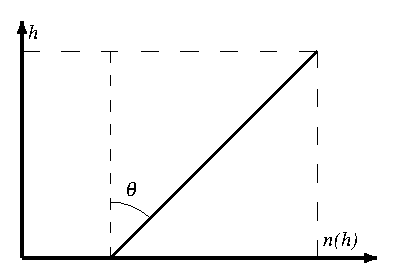
\includegraphics[width=6cm]{pictexa}
\caption{Diagram of a straight line}
\label{fig:line}
\end{center}
\end{figure}

Examples of references and a bibliography follow the acknowledgements.

\section*{Acknowledgements}

We wish to thank A.N. Colleague for enlightening comments on
the present topic.

\begin{thebibliography}{99}
\bibitem{Raby1966}
J.M. Raby, Biophysical aspects of radiation quality, International 
Atomic EnergyAgency, Technical Reports Series No. 58 (1966).
\bibitem{Dupont1961}
J.-P. Dupont, Proc. Int. Conf. on Radiation Hazards, Columbia, 
1960 (Academic Press Inc., New York, 1961), Vol. II, p. 396.
\bibitem{Appleman1959}
H. Appleman \emph{et al.}, J. \emph{Med. Biol.} \textbf{8} (1959) 911.
\bibitem{vanBerg1965}
E. van Berg, D. Johnson and J. Smith, \emph{Rad. Res.} \textbf{5} (1965) 
215.
\bibitem{Bryant1985}
Proceedings of the CAS--ECFA--INFN Workshop: The Generation of High Fields for Particle Acceleration to very High Energies, Frascati, Italy, September 1984, edited by P. Bryant and S. Newman, CERN--1985--007 (CERN, Geneva, 1985).\\
\url{https://doi.org/10.5170/CERN-1985-007}.
\bibitem{Allen1977}
M.A. Allen \emph{et al.}, \emph{IEEE Trans. Nucl. Sci.} \textbf{NS--24} (1977) 
1780.
\bibitem{cernrep}
Publishing Service, Preparing contributions to CERN Yellow Reports series,\\
\url{http://publishing.web.cern.ch/files/templates/CYR/LaTeX/cernrep.pdf}.
\end{thebibliography}

\section*{Bibliography}


I.C. Percival and D. Richards, \emph{Introduction to Dynamics}
(Cambridge University Press, Cambridge, 1982).

\appendix
\section{Title of appendix}
\label{sec:app}

\subsection{Subsection title in appendix}

Inside an appendix the same level of headings (section, subsection,
etc.) as in the main text applies. Only the first number is replaced
by an uppercase letter.

\subsubsection{Subsubsection title in appendix}

Inside a subsubsection inside an appendix.

\subsubsubsection{Subsubsubsection title in appendix}

\end{document}
